\documentclass{article}
\usepackage{template/spconf}
\usepackage[T1]{fontenc} 
\usepackage[utf8]{inputenc}
\usepackage[english]{babel}


\usepackage{template/clrscode3e}
\usepackage{color}
\usepackage[usenames,dvipsnames]{xcolor}
\usepackage[bookmarks=false, hidelinks]{hyperref}
\usepackage{graphicx}
\usepackage[tableposition=top]{caption}
\usepackage{subcaption}
\usepackage{amsmath}
\usepackage{amssymb}
\usepackage{breqn}
\usepackage{pgfplots}
\usepackage{tikz}
\usepackage{array}
\usepackage{hhline}
\usepackage{numprint}
\usepackage{microtype}

\usetikzlibrary{matrix}
\usetikzlibrary{arrows}

 
\usepackage{mathtools}
\DeclarePairedDelimiter{\floor}{\lfloor}{\rfloor}
\DeclarePairedDelimiter{\ceil}{\lceil}{\rceil}

\hypersetup{
    colorlinks=true,
    linkcolor=black,
    citecolor=black,
    filecolor=black,
    urlcolor=black,
}

\pgfplotsset{compat=1.8}


\hyphenpenalty=5000
\tolerance=1000
\emergencystretch=10pt

\newcommand{\beq}{\begin{dmath}}
\newcommand{\eeq}{\end{dmath}}
\newcommand{\beqs}{\begin{aligned}}
\newcommand{\eeqs}{\end{aligned}}

\newcommand{\x}{\mathbf{x}}
\newcommand{\hx}{\hat{\mathbf{x}}}
\newcommand{\B}{\mathbf{b}}
\newcommand{\R}{{R(\x)}}
\newcommand{\C}{\mathbf{c}}
\newcommand{\D}{D_p(\x)}
\newcommand{\SAD}{\text{SAD}}
\newcommand{\mGolomb}{G}
 
\newcommand{\vc}{\mathbf{c}}
\newcommand{\vx}{\mathbf{x}}
\newcommand{\vy}{\mathbf{y}}

\newcommand{\LM}{\lambda_{\text{\tiny{MOTION}}}}

\title{An Adaptive Search Ordering For Rate-Constrained Successive Elimination Algorithms}

\name{Luc Trudeau, Stéphane Coulombe, Christian Desrosiers\thanks{This work was funded by Vantrix Corporation and by the Natural Sciences and Engineering Research Council of Canada under the Collaborative Research and Development Program (NSERC-CRD 428942-11). Computations were made on the supercomputer Colosse from Université Laval, managed by Calcul Québec and Compute Canada. The operation of this supercomputer is funded by the Canada Foundation for Innovation (CFI), NanoQuébec, RMGA and the Fonds de recherche du Québec - Nature et technologies (FRQ-NT). Emails: \{luc.trudeau, stephane.coulombe, christian.desrosiers\}@etsmtl.ca
}}
\address{Department of Software and IT Engineering\\ École de technologie supérieure, Université du Québec\\ Montréal, Québec, Canada}

\begin{document}

\maketitle

%%%%%%%%%%%%%%%%%%%%%%%%%% ABSTRACT %%%%%%%%%%%%%%%%%%%%%%%%%%%
\begin{abstract}
This paper proposes a solution for the problem of unnecessary cost function evaluations, found when combining the successive elimination algorithm with a spiral scan search ordering. Our experiments show that the implementation of such a combination inside the HEVC reference software leads to unnecessary cost function evaluations. On the tested video sequences, an average of 3.46\% unnecessary cost function evaluations was measured. Considering only small block sizes (e.g., $4\!\times\!8$ and $8\!\times\!4$), this average rises to 8.06\%. To solve this problem, we propose an adaptive scan ordering of block matching candidates within the search area. When used with our early termination threshold, the proposed approach will only evaluate necessary cost functions, without impacting rate-distortion.
\end{abstract}

\begin{keywords}
\small{Successive elimination algorithms, Motion estimation, HEVC.}
\end{keywords}
%%%%%%%%%%%%%%%%%%%%%%%%%%%%%%%%%%%%%%%%%%%%%%%%%%%%%%%%%%%%%%%%

%%%%%%%%%%%%%%%%%%%%%%%%%% INTRODUCTION %%%%%%%%%%%%%%%%%%%%%%%%%%%
\vspace{-2mm}
\section{Introduction}
\label{sec:intro}
\vspace{-1mm}
In the context of video compression, motion estimation algorithms improve compression by exploiting spatiotemporal predictability. Given a cost function, they select the best candidate block from a search area in one or many anchor frames to serve as a predictor for the content of the current block. This operation is often referred to as block matching.

Recent demands for beyond-HD video formats (e.g., $4\text{K}$ or $8\text{K}$), the emergence of multiview video content, and feature-rich video compression standards are all factors that require video encoders to consider more block sizes, more anchor frames, and use bigger search areas~\cite{Sullivan2012}. Modern video encoders evaluate a much greater amount of block matching candidates than their former counterparts.  

The High Efficiency Video Coding (HEVC) standard~\cite{HEVC}, also known as H.265, is an example of a feature-rich video encoding standard. H.265/HEVC was designed to provide approximately 50\% bit-rate savings for equivalent perceptual quality when compared to the H.264/MPEG-4 AVC standard~\cite{H264}. However, it also contributes to a significant increase in the computational burden related to motion estimation. 

An Exhaustive Search Algorithm (ESA) performs motion estimation by evaluating the cost function for each block matching candidate inside the search area of every anchor frame. The high computational complexity incurred by evaluating the cost of all possible candidates allowed by the HEVC standard limits practical applications of the ESA in modern encoders.

Algorithms designed to reduce this computational complexity are classified according to whether or not they preserve optimality. Those that do not preserve optimality often rely on the assumption of a monotonically increasing match criterion around the location of the optimal candidate block. When this assumption does not hold, the accuracy of the motion estimation algorithm is reduced, as it will converge towards a local minimum. Modern algorithms in this class include zonal search algorithms \cite{Tourapis2000, Tourapis2002}, which first evaluate a set of predictors in order to constrain a local diamond or square search to a very narrow zone of the search area.

Optimality-preserving algorithms employ known inequalities to filter out block matching candidates. These inequalities allow to quickly determine the candidates whose cost functions cannot be smaller than that of the current best candidate. In this situation, evaluating the cost is unnecessary and only wastes computational resources. Recent algorithms in this class append more efficient filtering criteria to the successive elimination algorithm (SEA) proposed in~\cite{Li1995}. For example, \cite{Gao2000, Zhu2005a} propose to partition blocks to improve filtering efficiency.

An important fact, not considered in the work of Li and Salari~\cite{Li1995}, is that not all block matching candidates require the same amount of bits to encode their motion vector. Optimal encoding must consider not only the prediction accuracy of a candidate, but also the number of bits required to encode its vector. In encoding standard recommendations, the trade-off between prediction accuracy and motion vector cost is defined using the Lagrange multiplier ($\lambda$); the Lagrange multiplier is included in the motion estimation cost function, but is not taken into consideration by the original SEA algorithm. 

In~\cite{Coban1998}, Coban and Mersereau modified the SEA filtering criterion to take into account the number of bits required to encode the motion vector of a block matching candidate. This modification is in line with the HEVC encoder-side description of the test model reference software~\cite{McCann2014}, where the optimal matching candidate block is the best rate-constrained match.

The SEA filtering criterion can also be improved via the candidate search ordering used during motion estimation. Spiral search ordering outperforms raster search ordering by evaluating better block matching candidates earlier in the search process, which in turn filters out more block matching candidates. Spiral search ordering is considered state-of-the-art, and is used in many implementations of SEA-based algorithms~\cite{Zhu2005a, Coban1998, Yang2004}. However, Trudeau et al.~\cite{Trud14} showed that a spiral search ordering, in a rate-constrained context, will perform unnecessary cost function evaluations. To avoid this, the motion vector cost of the search ordering must increase monotonically, otherwise the SEA filtering criterion is weakened.

In this paper, we extend the work of \cite{Li1995}, \cite{Coban1998} to support the H.265/HEVC standard and implement it in the HEVC reference software. However, as described in \cite{Trud14}, this leads to unnecessary cost function evaluations. To resolve this problem, we propose an approach to adapt the search ordering of block matching candidates. We also describe a motion estimation algorithm that can adapt the search ordering, and when combined with the proposed early termination threshold, will only perform necessary cost function evaluations. To our knowledge, this is the first time a motion estimation algorithm capable of only performing necessary cost function evaluations is proposed. The result of this motion estimation algorithm is the same as with the ESA.

This paper is organized as follows: Section~\ref{sec:rdsea} describes the rate-constrained successive elimination and motivates the need for rate-constrained search orderings. The proposed dynamic approach to generate an adaptive search ordering is presented in \autoref{sec:searchOrder}. In \autoref{sec:results}, the experimental procedure and results are discussed. Finally, a summary of the contributions of this work and results are given in \autoref{sec:conclusion}.
%%%%%%%%%%%%%%%%%%%%%%%%%%%%%%%%%%%%%%%%%%%%%%%%%%%%%%%%%%%%%%%%


%%%%%%%%% Rate-Constrained Successive Elimination Algorithms %%%%%%%%
\vspace{-2mm}
\section{Rate-Constrained Successive Elimination Algorithms}
\label{sec:rdsea}
\vspace{-1mm}
The Successive Elimination Algorithms (SEA) use the triangle inequality to filter out block matching candidates whose cost function cannot be lower than the current cost of the best block matching candidate. This leads to computational savings of 85\% when compared to ESA\cite{Li1995}.

The inequality proposed in~\cite{Li1995} is written as:
\beq
\small
| \sum{B} - \sum{C(\vx_i,\vy_i)} | \leqslant \sum{|B - C(\vx_i,\vy_i)|} \:,
\label{eq:SEA}
\eeq 
where $B$ is a matrix of the pixel values inside the current block and $C(\vx_i,\vy_i)$ is a matrix of the pixel values of the $i$th candidate block located at position $(\vx_i,\vy_i)$ in the search area. We will refer to the left hand side of this equation as the absolute difference of sums (ADS). 

The right hand side contains the sum of the absolute differences (SAD) between the pixel values of the current block and those of the $i$th candidate block.

While the complexity of computing $\sum{B}$ and $\sum{C(\vx_i,\vy_i)}$ might appear to be equivalent to that of computing $\sum{|B - C(\vx_i,\vy_i)|}$, using the fast calculation of block sums proposed in~\cite{Li1995}, $B$ and $C(\vx_i,\vy_i)$ are precomputed and only require table lookups during motion estimation. As explained in~\cite{Li1995}, the overhead for precaculating these sums is negligible when compared to the savings gained.

In~\cite{Coban1998}, Coban and Mersereau added the rate constraint to the successive elimination algorithms. In a rate-constrained video encoder, this constraint must be added to the SEA in order to produce correct results. Failure to do so could impair the motion estimation module. They also found that the constraint produced a more effective filtering. The rate-constrained inequality is defined as:
\beq
\small
\begin{aligned}
| & \sum{B} - \sum{C(\vx_i,\vy_i)} | + \lambda R(\vx_i,\vy_i) \\ \leqslant
& \sum{|B - C(\vx^*_{i-1},\vy^*_{i-1})|} + \lambda R(\vx^*_{i-1},\vy^*_{i-1}) \:,
\end{aligned}
\label{eq:RDSEA}
\eeq
where $\lambda$ is the Lagrange multiplier (for the HEVC standard, the recommended function to compute $\lambda$ is described in~\cite{McCann2014}). The $R(x,y)$ function, often referred to as the rate, returns the number of bits required to encode the motion vector of the block matching candidate at position $(x,y)$. The term $(\vx^*_{i}, \vy^*_{i})$ is the current best candidate, considering the candidates from 0 to $i-1$ in the search ordering, and is such that:
\beq
\small
\begin{aligned}
\forall n \in \{0,\ldots,i\} & \Bigl( \sum{|B - C(\vx^*_{i},\vy^*_{i})|} + \lambda
R(\vx^*_{i},\vy^*_{i}) \\ 
\leqslant & \: \sum{|B - C(\vx_{n},\vy_{n})|} + \lambda
R(\vx_{n},\vy_{n})\Bigr)\:.
\end{aligned}
\eeq
%%%%%%%%%%%%%%%%%%%%%%%%%%%%%%%%%%%%%%%%%%%%%%%%%%%%%%%%%%%%%%%%%%%%


%%%%%%%%%%%%%%%%%%%%% Adaptive Search Ordering% %%%%%%%%%%%%%%%%%%%%
\section{Adaptive Search Ordering}
\label{sec:searchOrder}
Implementing the successive elimination algorithm combined with a spiral search ordering in the H.265/HEVC HM reference software can considerably reduce --~but not eliminate~-- unnecessary cost function evaluations. For example, a spiral search ordering applied to a bad predicted motion vector would cause multiple unnecessary cost function evaluations. Even with a good motion vector prediction, the spiral ordering does not follow the monotonically increasing rate rule defined in~\cite{Trud14}. This will lead to unnecessary cost function evaluations as the SEA threshold in equation~\ref{eq:RDSEA} will vary according to the difference in rate between the best block matching candidate and the current candidate.

While exponential Golomb codes are no longer used to encode motion vectors, the method proposed by Trudeau et al.~\cite{Trud14} for H.264 can be extended to HEVC. In HEVC, the bit length of the exponential Golomb encoding of the motion vector is recommended as a fast estimate of the motion vector cost for the rate-constrained motion estimation algorithm (as seen in the HEVC reference software~\cite{McCann2014}).

The new class of search orderings, proposed in~\cite{Trud14}, also known as rate-constrained search orderings, are based on the monotonically increasing rate rule

\beq
\small
R(\vx_i, \vy_i) \geqslant R(\vx_{i-1}, \vy_{i-1})\:.
\label{eq:SearchOrdering}
\eeq

This rule states that block matching candidates must be evaluated by increasing order of motion vector bit length, hence the name rate-constrained search ordering. We can see from \autoref{fig:ExpGolomb2D} that multiple search orderings can be derived from this rule, as the ordering of candidates with the same motion vector bit length can be intermixed. 

\begin{figure}[htb] \centering
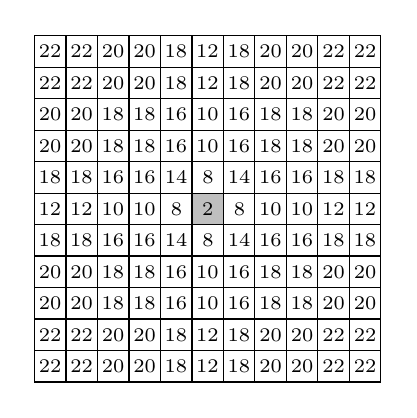
\begin{tikzpicture}
\tikzset{square matrix/.style={
    matrix of nodes,
    column sep=-\pgflinewidth, row sep=-\pgflinewidth,
    nodes={draw,
      minimum height=#1,
      anchor=center,
      text width=#1,
      align=center,
      inner sep=0pt
    },
  },
  square matrix/.default=0.4cm
}
\scriptsize{
\matrix[square matrix]{ & 22 & 22 & 20 & 20 & 18 &
12 & 18 & 20 & 20 & 22 & 22 \\ & 22 & 22 & 20 & 20 & 18 & 12 & 18 & 20 & 20 & 22 & 22 \\ 
& 20 & 20 & 18 & 18 & 16 & 10 & 16 & 18 & 18 & 20 & 20 \\
& 20 & 20 & 18 & 18 & 16 & 10 & 16 & 18 & 18 & 20 & 20 \\
& 18 & 18 & 16 & 16 & 14 &  8 & 14 & 16 & 16 & 18 & 18 \\
& 12 & 12 & 10 & 10 &  8 &  |[fill=lightgray]|2 &  8 & 10 & 10 & 12 & 12 \\
& 18 & 18 & 16 & 16 & 14 &  8 & 14 & 16 & 16 & 18 & 18 \\
& 20 & 20 & 18 & 18 & 16 & 10 & 16 & 18 & 18 & 20 & 20 \\
& 20 & 20 & 18 & 18 & 16 & 10 & 16 & 18 & 18 & 20 & 20 \\
& 22 & 22 & 20 & 20 & 18 & 12 & 18 & 20 & 20 & 22 & 22 \\
& 22 & 22 & 20 & 20 & 18 & 12 & 18 & 20 & 20 & 22 & 22 \\};
}
\end{tikzpicture}
\caption{\small Motion vector bit lengths for the block matching candidates of a subset of the search area. The gray square is the predicted motion vector. Multiple rate-constrained search orderings are possible, as block matching candidates with the same motion vector bit length can be combined in any order.}
\label{fig:ExpGolomb2D}
\end{figure}

With multiple search orderings comes the question of which ordering is optimal, which is not trivial to answer. Because the efficiency of the search ordering is greatly influenced by the content of the video sequence.

A search is SEA-optimal if the cost function is evaluated only for the block matching candidates such that
\beq
\small
\begin{aligned}
| & \sum{B} - \sum{C(\vx_i,\vy_i)} | + \lambda R(\vx_i,\vy_i) \\ \leqslant
& \sum{|B - C(\hat{\vx},\hat{\vy})|} + \lambda R(\hat{\vx},\hat{\vy}) \:,
\end{aligned}
\label{eq:RDSEAOptimal}
\eeq 

where $(\hat{\vx},\hat{\vy})$ is the best candidate over the entire search area. Thus, the search is SEA-optimal if the number of cost function evaluations is equal to the number of block matching candidates, where the rate-constrained ADS (RCADS) is less than the best rate-constrained SAD (RCSAD) found inside the search area (only those candidates have a chance to be optimal). Indeed, because of equation~\ref{eq:SEA}, it is unnecessary to evaluate candidates that do not meet equation~\ref{eq:RDSEAOptimal}. Furthermore, although we do not know the best candidate needed to apply equation~\ref{eq:RDSEAOptimal}, the $\proc{MotionEstimation}$ function is our proposed adaptive method for an SEA-optimal search.

The parameters of the $\proc{MotionEstimation}$ function are: $\textbf{B}$, the image to encode; $\textbf{C}$, the anchor frame; $(\id{bx},\id{by})$, the block coordinates; $\id{ord}$, the search ordering; $\textbf{sB}$, the sum buffer of $\textbf{B}$, and $\textbf{sC}$, the sum buffer of the $\textbf{C}$. 

By using table lookups (lines~\ref{li:tableLookup1} and \ref{li:tableLookup2}), we can determine the RCADS (line~\ref{li:rcads}) of each block matching candidate in the search area. The candidates are then sorted by increasing value of RCADS (line~\ref{li:Sort}). Starting with the lowest RCADS candidate, we successively evaluate the cost function until the later exceeds the lowest cost (lines~\ref{li:Threshold1}-\ref{li:Threshold2}), at which point evaluating the cost function of the remaining block matching candidate becomes irrelevant (because of equation~\ref{eq:RDSEA}). This procedure is SEA-optimal because no candidate for which RCADS is higher than the best cost is evaluated (this is obvious from the RCADS-sorted scan order). It is also obvious that the proposed procedure ensures that the optimal value is found.

\begin{codebox}
\Procname{$\proc{MotionEstimation}(\textbf{B}, \textbf{C}, \id{bx}, \id{by}, \id{ord}, \textbf{sB}, \textbf{sC})$}
\li $\id{sumB} \gets \textbf{sB}[\id{bx}][\id{by}]$ \label{li:tableLookup1}
\li $x \gets \attrib{ord[0]}{x}$
\li $y \gets \attrib{ord[0]}{y}$
\li $\id{bestCost} \gets \proc{SAD}(\textbf{B}, \textbf{C}, \id{bx}, \id{by}, x, y) + \lambda \times \proc{R}(x,y)$ \label{li:MVP}
\li $\id{bestVector} \gets \id{ord[0]}$
\li $numCont \gets 0$
\li \For $i \gets 1$ \To $\attrib{ord}{length} - 1$
\li \Do
      $x \gets \attrib{ord[i]}{x}$
\li   $y \gets \attrib{ord[i]}{y}$
\li   $\id{sumC} \gets \textbf{sC}[\id{bx} + x][\id{by} + y]$ \label{li:tableLookup2}
\li   $\id{vCost} \gets \lambda \times \proc{R}(x,y)$
\li   $\id{rcasd} \gets | \id{sumB} - \id{sumC} | + \id{vCost}$ \label{li:rcads}
\li   \If $\id{rcasd} \leqslant \id{bestCost}$ \label{li:prune1}
\li   \Then
        $\id{cont[\id{numCont}]} \gets (\id{rcasd}, x, y, \id{vCost})$ \label{li:prune2}
\li     $\id{numCont} \gets \id{numCont} + 1$
      \End
    \End
\li $\id{cont} \gets \proc{Sort}(\id{cont})$ \label{li:Sort}
\li \For $i \gets 0$ \To $\id{numCont} - 1$
\li \Do
      $\id{rcasd} \gets \attrib{cont[i]}{rcasd}$
\li   \If $\id{rcasd} > \id{bestCost}$ \label{li:Threshold1}
\li   \Then
        \Return $\id{bestVector}$ \label{li:Threshold2}
\li   \Else
\li
        $x \gets \attrib{cont[i]}{x}$
\li     $y \gets \attrib{cont[i]}{y}$
\li     $cost \gets \attrib{cont[i]}{vCost}$
\li     $\id{cost} \gets \id{cost} + \proc{SAD}(\textbf{B}, \textbf{C}, \id{bx}, \id{by}, x, y)$
\li     \If $\id{cost} < \id{bestCost}$
\li     \Then
          $\id{bestCost} \gets \id{cost}$
\li       $\id{bestVector} \gets (x,y)$
        \End
      \End
    \End
\end{codebox}

We can further reduce the processing complexity by pruning the block matching candidates that will be sorted (lines~\ref{li:prune1}-\ref{li:prune2}). Assuming that we evaluate the cost function of a candidate, by applying its cost in equation~\ref{eq:RDSEA}, we can filter out candidates with higher RCADS. The closer the cost function is to the best cost, the better the filter will be. For convenience, we will use the cost function of the predicted motion vector (line \ref{li:MVP}) as an upper bound in equation~\ref{eq:RDSEAOptimal} to replace the best cost (which is unknown). In the worst case, the predictor will not be effective, and all candidates will need to be sorted. However, this will not affect the number of cost function evaluations (just the number of candidates to sort, which has a small impact on performance).
%%%%%%%%%%%%%%%%%%%%%%%%%%%%%%%%%%%%%%%%%%%%%%%%%%%%%%%%%%%%%%%%%%%%%


%%%%%%%%%%%%%%% Experimental results and discussion %%%%%%%%%%%%%%%%%
\section{Experimental results and discussion}

\label{sec:results}
To test our hypotheses, we implemented the rate-constrained SEA with a spiral scan search ordering and the proposed approach in the H.265/HEVC HM 13.1 reference software~\cite{McCann2014}. By comparing the cost function evaluation of both approaches, we could determine the percentage of unnecessary cost function evaluations performed by the RCSEA with a spiral search ordering.

Table~\ref{tab:SADGain} presents detailed results of our experiment for the first 100 frames of standard Class C ($832\!\times\!480$) video sequences (``\textit{Basketball Drill}'', ``\textit{Party Scene}'', ``\textit{BQ Mall}'' and ``\textit{Race Horses}''). The results are presented by block sizes and by QP values. We used the main profile with the following alterations: 5 reference frames, disabled asymmetric motion partitions, full pixel precision motion estimation and full search motion estimation.

\begin{table}[htb]                              
\centering
\small
  \caption{\small Percentage of unnecessary cost function evaluations made by a rate-constrained SEA with a spiral scan search ordering in the H.265 HM reference software compared to the proposed method}                      
\label{tab:SADGain}                       
\begin{tabular}{|l|c|c|c|c|c|}                 
\hline   
Block Size & QP & Basket & Party & Mall & Horses\\  
\hline                               
$4\times 8$, $8\times 4$ & 22 & 8.29 & 5.58 & 3.35 & 7.59 \\    
\hline                                         
$8\times 8$ & 22 & 4.74 & 3.56 & 2.33 & 6.34 \\        
\hline                                         
$8\times 16$, $16\times 8$ & 22 & 3.59 & 2.60 & 1.66 & 5.97 \\  
\hline                                         
$16\times 16$ & 22 & 3.22 & 2.15 & 1.23 & 5.80 \\      
\hline                                         
$16\times 32$, $32\times 16$ & 22 & 2.94 & 1.94 & 0.96 & 5.44 \\
\hline                                         
$32\times 32$ & 22 & 2.61 & 1.60 & 0.77 & 4.93 \\      
\hline                                         
$32\times 64$, $64\times 32$ & 22 & 2.14 & 1.18 & 0.60 & 3.87 \\
\hline                                         
$64\times 64$ & 22 & 1.89 & 0.60 & 0.31 & 2.89 \\      
\hline \hline                                         
$4\times 8$, $8\times 4$ & 27 & 10.99 & 6.73 & 3.25 & 8.46 \\   
\hline                                         
$8\times 8$ & 27 & 5.94 & 4.33 & 2.14 & 6.49 \\        
\hline                                         
$8\times 16$, $16\times 8$ & 27 & 3.56 & 3.01 & 1.53 & 5.79 \\  
\hline                                         
$16\times 16$ & 27 & 2.87 & 2.21 & 1.16 & 5.50 \\      
\hline                                         
$16\times 32$, $32\times 16$ & 27 & 2.57 & 1.91 & 0.93 & 5.18 \\
\hline                                         
$32\times 32$ & 27 & 2.23 & 1.58 & 0.75 & 4.73 \\      
\hline                                         
$32\times 64$, $64\times 32$ & 27 & 1.81 & 1.16 & 0.56 & 3.79 \\
\hline                                         
$64\times 64$ & 27 & 1.62 & 0.61 & 0.31 & 2.88 \\      
\hline \hline                                         
$4\times 8$, $8\times 4$ & 32 & 13.12 & 7.95 & 3.30 & 10.10 \\  
\hline                                         
$8\times 8$ & 32 & 7.78 & 4.99 & 1.97 & 6.99 \\        
\hline                                         
$8\times 16$, $16\times 8$ & 32 & 4.39 & 3.30 & 1.38 & 5.86 \\  
\hline                                         
$16\times 16$ & 32 & 2.89 & 2.29 & 1.06 & 5.42 \\      
\hline                                         
$16\times 32$, $32\times 16$ & 32 & 2.51 & 1.83 & 0.88 & 5.10 \\
\hline                                         
$32\times 32$ & 32 & 2.14 & 1.46 & 0.72 & 4.62 \\      
\hline                                         
$32\times 64$, $64\times 32$ & 32 & 1.76 & 1.07 & 0.52 & 3.80 \\
\hline                                         
$64\times 64$ & 32 & 1.46 & 0.58 & 0.27 & 2.79 \\      
\hline \hline                                         
$4\times 8$, $8\times 4$ & 37 & 15.35 & 9.19 & 3.31 & 12.45 \\  
\hline                                         
$8\times 8$ & 37 & 9.06 & 5.51 & 1.84 & 7.33 \\        
\hline                                         
$8\times 16$, $16\times 8$ & 37 & 5.19 & 3.43 & 1.21 & 5.50 \\  
\hline                                         
$16\times 16$ & 37 & 3.07 & 2.18 & 0.90 & 4.93 \\      
\hline                                         
$16\times 32$, $32\times 16$ & 37 & 2.30 & 1.68 & 0.78 & 4.66 \\
\hline                                         
$32\times 32$ & 37 & 1.93 & 1.29 & 0.66 & 4.27 \\      
\hline                                         
$32\times 64$, $64\times 32$ & 37 & 1.61 & 0.98 & 0.50 & 3.46 \\
\hline                                         
$64\times 64$ & 37 & 1.37 & 0.49 & 0.28 & 2.72 \\      
\hline
\end{tabular}                                            
\end{table}

As stated in \cite{Trud14}, changing the search ordering has negligible to no impact on rate-distortion as all candidates are considered, only in a different order. 

From the results in table~\ref{tab:SADGain}, we can see that the proposed algorithm is more effective for smaller block sizes. This is due to the fact that smaller blocks comprise fewer pixels, which leads to more precise ADS values. These values filter out more unnecessary cost function evaluations. Since most SEA-based algorithms partition bigger blocks using multiple small partitions to improve filtering efficiency~\cite{Gao2000, Zhu2005a, Yang2004, Toivonen2004}, they would benefit significantly from the proposed method.

As the QP increases, the effectiveness of the proposed algorithm also increases. This is analogous to the findings of \cite{Coban1998}, and is caused by an increase in the value of the Lagrange multiplier. This in turn increases the ratio between the weighted number of bits required to encode the motion vector and the prediction error. When this occurs, the rate constraint becomes more significant and allows more block matching candidates to be filtered.

\autoref{tab:SADGain} shows that the proposed search ordering is, on average, more efficient with sequences that contain important and unpredictable movement (``\textit{Basketball Drill}'' and ``\textit{Race Horses}''),  than with those with more predictable sequences. Unpredictable sequences lead to less precise motion vector predictions, and for them, hard-coded search orderings, such as spiral scan, will search around a bad starting point leading to unnecessary cost function evaluations. In the same context, by sorting block matching candidates, the proposed adaptive approach exploits the relative precision of the RCADS, allowing candidates around the true motion vector to be considered earlier in the search process.

%%%%%%%%%%%%%%%%%%%%%%%%%%%%%%%%%%%%%%%%%%%%%%%%%%%%%%%%%%%%%%%

%%%%%%%%%%%%%%%%%%%%%%%%% Conclusion %%%%%%%%%%%%%%%%%%%%%%%%%%
\section{Conclusion}
\label{sec:conclusion}
In this paper, we proposed an algorithm that can dynamically adapt the search ordering of the motion estimation module, and an early termination threshold that guarantees to only perform necessary cost function evaluations. Our experiments show that, without our algorithm, an implementation of the rate-constrained successive elimination algorithm using a spiral scan search ordering in the H.265/HEVC HM reference software would lead to an average of 3.5\% unnecessary cost function evaluations. In some instances, the proposed method can reduce the percentage of cost function evaluations up to 15\%.
%%%%%%%%%%%%%%%%%%%%%%%%%%%%%%%%%%%%%%%%%%%%%%%%%%%%%%%%%%%%%%%%

\bibliographystyle{template/IEEEtran}
\bibliography{refs}

\end{document}